\message{ !name(capitolo2.tex)}
\message{ !name(capitolo2.tex) !offset(-2) }
\chapter{Stato dell'arte}
\label{capitolo2}
\thispagestyle{empty}

%\begin{quotation}
%{\footnotesize
%\noindent{\emph{``Terence: Tu lo reggi il whisky? \\
%Bud: Beh, i primi due galloni si, al terzo divento nostalgico e ci pu\`o scappare la lite... E tu lo reggi? \\
%Terence: Eh, che domande, io sono stato allattato a whisky!''
%} }
%\begin{flushright}
%I due superpiedi quasi piatti
%\end{flushright}
%}
%\end{quotation}
\vspace{0.5cm}


\noindent Nei paragrafi che seguono entriamo nel merito delle principali aree di ricerca su cui il presente lavoro \`e basato.
Nel primo paragrafo analizziamo quali sono le tecniche principalmente utilizzate per identificare un cambiamento all'interno di un processo stocastico, in particolare quando si hanno situazioni di \textit{non stazionariet\`a}. Nel secondo paragrafo vediamo le principali tecniche per la segmentazione di dati in sottoinsiemi e come possono essere applicate nella segmentazione di immagini e video.
Infine elenchiamo i principali algoritmi presenti in letteratura utilizzati nell'identificazione di quei fenomeni che compromettono la qualit\`a dell'acquisizione di una camera di video sorveglianza.
\section{Identificazione del cambiamento nella stazionariet\`a di un
  processo}
Una caratteristica, richiesta in molte applicazioni di analisi e processamento intelligente di dati, riguarda l'assunzione che il processo generante questi dati non cambi nel tempo \cite{alippi2014intelligence}. In questo caso si parla di processi \textit{stazionari}, ovvero processi dove i dati possono essere considerati generati da un'unica distribuzione probabilistica. \\
In molte situazioni, soprattutto se vengono utilizzati dei sensori per
misurare delle grandezze fisiche, si pu\`o incorrere in situazioni in
cui questa ipotesi di stazionariet\`a viene meno. Ad esempio, pu\`o
succedere che il sensore si guasti, oppure che fenomeni esterni non
permettano un'acquisizione ottimale. In questi casi \`e opportuno
avere a disposizione degli strumenti in grado di identificare quando
la condizione di stazionariet\`a di un processo viene meno, in modo da
poter lanciare un avviso a riguardo oppure dei metodi di
autoconfigurazione. Le tecniche principalmente utilizzate prendono il
nome di \textit{Change-Point Methods} (CPM) e \textit{Change-Detection
  Tests} (CDT), che verranno coperte nel resto del paragrafo.
\subsection{Metodi di Change-Point}
I metodi di Change-Point (CPM) vengono utilizzati per ispezionare una certa sequenza di dati e verificare la sua stazionariet\`a. Ci\`o viene fatto verificando che, all'interno della sequenza, esista un istante temporale in cui la distribuzione dei dati cambia (\textit{change point}).\\
In maniera formale possiamo dire che, data una sequenza di dati
\cite{alippi2014intelligence,ross2011nonparametric}
\[X=\{x(t), t = 1,...,n\},\]
essa contiene un change point all'istante $\tau < n$ se \`e possibile
suddividerla in due sottosequenze
\[ A_\tau = \{x(t), t = 1,...,\tau \}\]
\[ B_\tau = \{x(t), t = \tau + 1,...,n \},\]
le quali sono due realizzazioni \textit{indipendenti e identicamente
  distribuite} (i.i.d.) di due differenti variabili aleatorie con
distribuzione $ F_0 $ e $ F_1 $.
\`E possibile, quindi,  convertire il problema del change point in uno equivalente dove si valuta se $ A_\tau $ e $ B_\tau $ sono generati da due distribuzioni diverse.\\
Il problema, a questo punto, pu\`o essere riformulato come un
\textit{test d'ipotesi a due campioni} \cite{ross2009introduction},
dove l'\textit{ipotesi nulla} ($ H_0 $) e l'\textit{ipotesi
  alternativa} ($ H_1 $) sono le seguenti:
			
			\begin{eqnarray}
                          H_0: \quad  x(t) \sim F_0 \quad  \forall t \\
                          H_1: \quad  x(t) \sim 
                          \begin{cases}
                            F_{0} & \text{se } t < \tau, \\
                            F_{1} & \text{se } t \geq \tau
                          \end{cases}.
			\end{eqnarray}
			

			Per la valutazione delle ipotesi fatte sopra,
                        occorrono delle opportune \textit{statistiche
                          di test a due campioni}
                        \cite{ross2009introduction}
			
			\[ T_\tau = T(A_\tau, B_\tau), \]
			
			in modo da poter comparare $ A_\tau $ e $ B_\tau $ \cite{alippi2014intelligence}. In questo modo \`e possibile rifiutare l'ipotesi nulla quando il valore della statistica $ T_\tau $ supera una certa soglia $ h_{n,\alpha} $, calcolata in funzione di un certo \textit{intervallo di confidenza} $ \alpha $ e del numero di campioni $ n $.\\
			Se, ad esempio, consideriamo l'ipotesi che $
                        A_\tau $
                        e $ B_\tau $ siano generate da due
                        distribuzioni \textit{gaussiane}, \`e
                        possibile valutare la dissimilarit\`a tra le
                        due distribuzioni controllando i due
                        \textit{valori attesi}. Possiamo usare, come
                        statistica di test, la \textit{differenza
                          standardizzata tra le medie di due
                          campioni}, definita come
			
			\[ D_\tau = \sqrt{\frac{\tau(n-\tau)}{n}}
                        \frac{\overline{A}_\tau-\overline{B}_\tau}{S_\tau}, \]
			
			dove $ \overline{A}_\tau $ e $ \overline{B}_\tau $ denotano le \textit{medie compionarie} valutate rispettivamente su $ A_\tau $ e $ B_\tau $, mentre $ S_\tau $ \`e la \textit{varianza campionaria} valutata \textit{su tutto l'insieme dei dati}.\\
			
			Quando la statistica di test utilizzata,
                        corrispondente a una specifica partizione
                        dell'insieme dei dati, non fornisce l'evidenza
                        necessaria a rifiutare $ H_0, $ l'unica cosa
                        che \`e possibile stabilire \`e che
                        nell'istante $ \tau $ scelto non si \`e avuto
                        un cambiamento nella stazionariet\`a
                        dell'insieme. \textit{Ci\`o non implica che
                          l'istante di cambiamento non sia un altro
                          ancora da valutare.} In maniera rigorosa \`e
                        necessario valutare, quindi, tutte le
                        possibili partizioni dell'insieme dei dati
                        considerati. Le ipotesi nulla e alternativa
                        vengono, perci\`o, modificate nel seguente
                        modo \cite{ross2011nonparametric}:
			
			
			\begin{eqnarray}
                          H_0 : \forall t, & x(t) \sim F_0 \\
                          H_1 : \exists \tau & x(t) \sim 
                                               \begin{cases}
                                                 F_{0} & \text{se } t < \tau, \\
                                                 F_{1} & \text{se } t
                                                 \geq \tau
                                               \end{cases}.
			\end{eqnarray}
			
			Entrando pi\`u nel dettaglio, per ciascun
                        punto $ s \in \{2,...,n-1\} $, candidato a
                        essere un change point, valutiamo la
                        statistica di test $ T_s. $ Viene scelto come
                        change point quello che massimizza la
                        statistica
			\[ M= \argmax_{s=2,...,n-1} (T_s), \]
                        corrispondente al valore $ T_M $ di $T$
                        \[ T_M = \max_{s=2,...,n-1} (T_s).\]
                        Una volta trovato $T_M$ il test va finalizzato
                        comparando questa statistica con la soglia
                        $ h_{n,\alpha}, $ in modo da verificare se
                        l'ipotesi nulla sia da scartare o meno.
			 
			 \begin{figure}
                           \centering
                           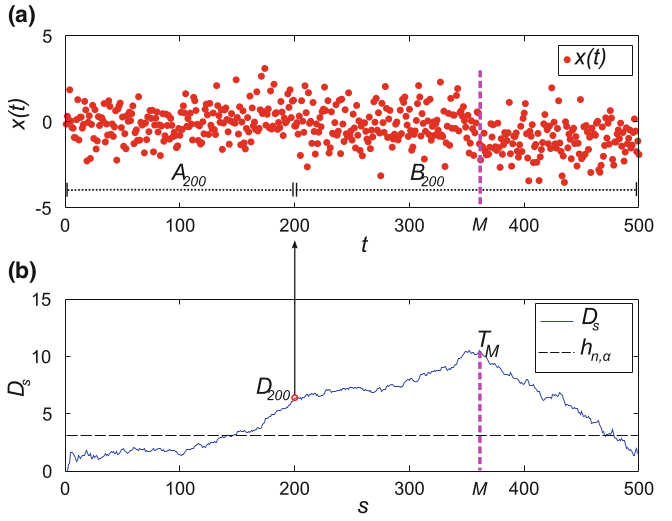
\includegraphics[width=12cm,keepaspectratio]{pictures/CPM}
                           \caption{Esempio di CPM}
                           \label{fig:CPM}
                         \end{figure}
			
                         Nella figura \ref{fig:CPM} possiamo vedere un esempio di CPM basato su una statistica \textit{t di Student} \cite{alippi2014intelligence}. La sequenza \`e formata da 500 dati (\textbf{a}) ed \`e stato individuato un cambiamento all'istante $\tau=350$. I valori delle varie statistiche in funzione di s sono visualizzati in (\textbf{b}).\\
			
                         Spesso \`e preferibile utilizzare dei test
                         statistici \textit{non parametrici},
                         soprattutto quando le distribuzioni dei dati
                         sono incognite. Le statistiche maggiormente
                         utilizzate sono quelle basate su
                         \textit{calcolo del rango}
                         \cite{ross2011nonparametric}. Quando si ha a
                         che fare con cambiamenti nella
                         \textit{localit\`a} dei dati una statistica
                         solitamente utilizzata \`e quella di
                         \textit{Mann-Whitney}, mentre quando si
                         vogliono verificare cambiamenti \textit{di
                           scala} \`e possibile utilizzare la
                         statistica di \textit{Mood}. La statistica di
                         \textit{Lepage} invece pu\`o risultare utile
                         per analizzare entrambi i tipi di
                         cambiamento. Un altro approccio consiste nel
                         comparare le \textit{distribuzioni empiriche}
                         dei due insiemi di dati, usando ad esempio la
                         statistica di \textit{Kolmogorov-Smirnov}.
			 
		\subsection{Change-Detection Test}
		I metodi di change point sono stati principalmente
                pensati per essere eseguiti \textit{a valle} della
                completa acquisizione dei dati. Inoltre il suo elevato
                costo computazionale fa s\`i che questa tecnica
                difficilmente possa essere utilizzabile all'interno di
                un sistema embedded. Le tecniche che vengono descritte
                in questo paragrafo, che prendono il nome di
                \textit{change detection test} (CDT), hanno come scopo
                principale quello di fare un processamento dei dati
                \textit{in linea}, ovvero non appena questi sono
                disponibili. Tecniche di questo tipo vengono anche
                chiamate \textit{tecniche sequenziali}. La loro
                relativa semplicit\`a dal punto di vista
                computazionale permette di utilizzarle all'interno di
                sistemi embedded ma, rispetto alle tecniche basate su
                CPM, abbiamo una latenza (ovvero l'intervallo di tempo
                tra l'istante di identificazione del cambiamento e
                quello in cui effettivamente questo \`e avvenuto) e un
                numero di falsi positivi (viene segnalato un
                cambiamento nella distribuzione quando in, realt\`a,
                questo non \`e avvenuto) maggiori.
                \subsubsection{Famiglia dei CDT basati su CUSUM}
                Le \textit{carte di controllo per le somme cumulate} (CUMulative SUM control chart, abbreviate in \textit{CUSUM}) \cite{alippi2014intelligence,ross2009introduction} permettono di identificare un cambiamento all'interno di una sequenza di dati in maniera molto accurata utilizzando alcune informazioni \textit{a priori} sul processo generante i dati. Queste informazioni vengono generalmente acquisite durante un \textit{fase di configurazione} del test, in modo da fissare i parametri di test necessari all'analisi.\\
                Nel seguito presentiamo due metodi di CDT che
                estendono il metodo CUSUM tradizionale rilassando
                alcune delle sue assunzioni troppo restrittive.  La
                prima variante permette di identificare in maniera
                automatica la configurazione dei parametri di test
                (\textit{CUSUM adattativo}), mentre la seconda,
                chiamata \textit{computational Intelligence CUSUM}
                (CI-CUSUM) \`e in grado di considerare un insieme
                pi\`u ricco di descrittori in modo da aumentare
                l'efficienza nell'identificare i cambiamenti
                \cite{alippi2008just}.  \subparagraph{CUSUM
                  tradizionale e versione adattativa}
                Sia \[X=\{x(t),t=1,...,N\},x(t)\in \mathbb{R}\]
                una sequenza di $N$ dati generata da un processo con
                densit\`a probabilistica $f_\theta(x)$, che assumiamo
                sconosciuta e parametrizzata secondo un vettore
                $\theta\in\mathbb{R}^n$. Assumiamo, inoltre, che il
                processo cambi la sua stazionariet\`a a un istante
                $T^0$ sconosciuto. Questo avvenimento pu\`o essere
                modellato come un passaggio dal vettore dei parametri
                $\theta_0$ a $\theta_1$, associati rispettivamente
                alle denit\`a $f_{\theta_0}(x)$ e
                $f_{\theta_1}(x)$. La discrepanza tra le due densit\`a
                viene valutata comparando il rapporto tra le
                log-verosimiglianze (\textit{log-likelihood ratio})
				
                \[
                s(t)=ln\frac{f_{\theta_1}(x(t))}{f_{\theta_0}(x(t))}
                \textit{ per ogni } t=1,...,N \]
							
                e la \textit{somma cumulata}
				
                \[ S(t) = \sum^t_{\tau=1} s(\tau) \]
				
                CUSUM identifica un cambiamento in $X$ all'istante $\widehat{T}$ quando \[g(t)=S(t)-m(t),\] ovvero la differenza tra il valore della somma cumulata all'istante $t$ e il suo valore minimo nel tempo \[m(t)=\min_{\tau=1,...,t}S(\tau),\] supera una certa soglia $h$.\\
				
                Il metodo CUSUM tradizionale assume che i parametri $\theta_0$, $\theta_1$ e la soglia $h$ siano disponibili a priori. La versione adattativa viene incontro a questa assunzione che, generalmente, \`e difficile da soddisfare.\\
                La variante prima di tutto genera la sequenza cumulata
                $Y=\{y(1),y(2),...\}$, dove $y(s)$ rappresenta il
                valore della media compionaria stimata su una
                \textit{finestra mobile non sovrapponibile} di
                ampiezza $n$ presa da $X$
				
                \[ y(s) = \frac{1}{n} \sum_{t=(s-1)n+1}^{sn}x(t) \]
				
                Scegliendo $n$ abbastanza grande, per il
                \textit{teorema del limite centrale}
                \cite{ross2009introduction}, la distribuzione di $Y$
                pu\`o essere approssimata con una distribuzione
                \textit{gaussiana}. In questo modo, quindi, si pu\`o
                utilizzare il metodo CUSUM tradizionale direttamente
                sulla sequenza $Y$. I primi $K$ dati di $X$ vengono
                usati come \textit{insieme di configurazione} per i
                parametri necessari a identificare il cambiamento. Il
                vettore dei parametri $\theta_0$ \`e caratterizzato da
                media e varianza di $Y$, stimate attraverso i primi
                $K/n$ campioni di $Y$. Il vettore dei parametri
                $\theta_1$ viene ottenuto attraverso l'identificazione
                di un intorno di confidenza per $\theta_0$, mentre la
                soglia $h$ viene calcolata come il valore massimo di
                $g(t)$ nella sequenza $Y$
				
                \[ h=\max_{1\leq t\leq N/n}g(t). \]
				
                \noindent L'intera procedura \`e illustrata nella
                figura \ref{fig:adaptiveCUSUM}.
				
				\begin{figure}
                                  \centering
                                  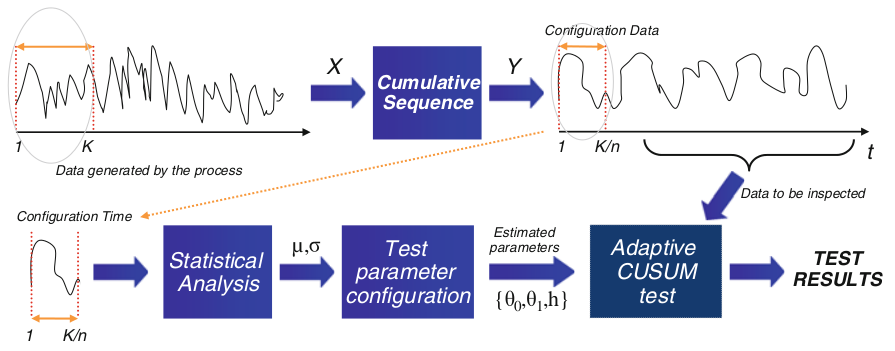
\includegraphics[width=12cm,keepaspectratio]{pictures/adaptiveCUSUM}
                                  \caption{Procedura del CUSUM
                                    adattativo}
                                  \label{fig:adaptiveCUSUM}
				\end{figure}
				
				\subparagraph{CI-CUSUM} Il metodo
                                CI-CUSUM rappresenta un'estensione del
                                CUSUM adattativo molto potente, in
                                quanto ciascun descrittore, estratto
                                dal flusso di dati, pu\`o essere
                                utilizzato per avere differenti gradi
                                di sensitivit\`a durante
                                l'identificazione di un cambiamento.
				
				\begin{figure}
                                  \centering
                                  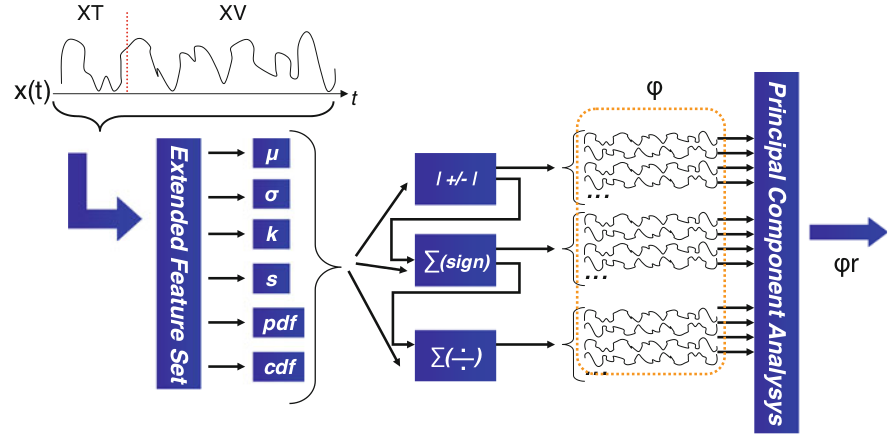
\includegraphics[width=12cm,keepaspectratio]{pictures/CI-CUSUM}
                                  \caption{Estrazione dei descrittori
                                    nel metodo CI-CUSUM}
                                  \label{fig:CI-CUSUM}
				\end{figure}
				
				Facciamo riferimento alla figura \ref{fig:CI-CUSUM}. I descrittori $\varphi$ considerati contengono i principali momenti della distibuzione dei dati, come media e varianza, ma anche momenti superiori al secondo come skewness (\textit{skew}) e kurtosis (\textit{kurt}), oltre che altre informazioni derivate dalla densit\`a probabilistica (\textit{pdf}) e dalla funzione di ripartizione dei dati (\textit{cdf}).\\
				A ogni istante queste grandezze
                                vengono confrontate con quelle
                                appartenenti all'intervallo di
                                configurazione (\textit{training set},
                                indicato in figura \ref{fig:CI-CUSUM}
                                come TS), in modo da valutare la
                                discrepanza tra questi valori. I
                                descrittori utilizzati sono
				\[
                                \varphi_1(t)=|\mu_0-\mu_V|,\varphi_2(t)=|\sigma_0-\sigma_V|,\]
				\[\varphi_3(t)=|\textit{kurt}_0-\textit{kurt}_V|,\varphi_4(t)=|\textit{skew}_0-\textit{skew}_V|, \]
				
				\[\varphi_5(t)=\int_x|\textit{pdf}_0(x)-\textit{pdf}_V(x)|\textit{dx},\]
				\[\varphi_6(t)=\int_x|\textit{cdf}_0(x)-\textit{cdf}_V(x)|\textit{dx}, \]
				
				\[ \varphi_{7\leq j\leq 12}(t)=
                                \sum_{v=1}^{t-1}\textit{sgn}(\varphi_{j-6}(v+1)-\varphi_{j-6}(v)),\]
				\[\varphi_{13\leq j\leq 24}(t)=
                                \sum_{v=1}^{t-1}\frac{\varphi_{j-12}(v+1)}{\varphi_{j-12}(v)} \]
				
				In particolare, i descrittori
                                $\varphi_5(t)$ e $\varphi_6(t)$
                                valutano la discrepanza tra la
                                densit\`a e funzione di ripartizione
                                correnti e quelle rispettive
                                dell'intervallo di configurazione. I
                                descrittori da $\varphi_7(t)$ a
                                $\varphi_{12}(t)$ vanno ad analizzare
                                i cambiamenti di segno in elementi
                                consecutivi e quelli da
                                $\varphi_{13}(t)$ a $\varphi_{24}(t)$
                                la somma cumulata del rapporto tra
                                elementi consecutivi. Per ridurre la
                                complessit\`a dello spazio dei
                                descrittori viene applicata
                                un'\textit{analisi delle componenti
                                  principali} su $\varphi$, in modo da
                                avere la trasformata $\varphi_r$. A
                                questo punto, dato che la
                                distribuzione di $\varphi_r$ non \`e
                                nota a priori, viene applicato un
                                CUSUM adattativo su di essa.
				
			        \subsubsection{Famiglia dei CDT basati
                                  su Intersezione di Intervalli di
                                  Confidenza}
                                
                                \subsubsection{CDT di tipo gerarchico}

	\section{Segmentazione di immagini e video}
	In molte applicazioni di visione artificiale \`e spesso necessario estrarre, da un'immagine o un video, una o pi\`u regioni specifiche. Quando si vanno a trattare dei video, i tipi di segmentazione che possono essere applicati sono solitamente due:
		\begin{itemize}      
			\item una segmentazione di tipo \textit{spaziale}, in cui vengono estratti dei pixel specifici per ogni frame costituente il video;
			\item una segmentazione di tipo \textit{temporale}, in cui vengono estratti dei frame 			significativi (\textit{key-frames}).
	\end{itemize}
	Segmentazioni di tipo spaziale permettono, ad esempio, di seguire il movimento di uno specifico oggetto all'interno della scena ripresa \cite{kim2003efficient}, mentre segmentazioni di tipo temporale permettono di dividere un filmato in \textit{shot} oppure di creare una sintesi del video con dei frame significativi. In quest'ultimo caso si parla di \textit{key-frames extraction} o di \textit{video summarization} \cite{gong2000video,jiang2009hierarchical,sentinelli2014live,wolf1996key}. Quando si vanno a trattare immagini la segmentazione \`e di tipo spaziale.\\
	Considerando la segmentazione di tipo spaziale, nella maggior parte dei casi la tecnica consiste nell'utilizzare dei descrittori per ciascun pixel e applicare delle tecniche di \textit{clustering}, ovvero delle metodologie atte a partizionare un insieme di dati \cite{han2006data}, sugli stessi. Nel seguito andiamo a vedere brevemente le caratteristiche principali della tecnica di clustering \textit{k-means}, guardando anche le metodologie utilizzate per determinare il numero ottimale di cluster, dopodich\`e vedremo alcune tecniche di segmentazione che sfruttano questo tipo di clustering.
		\subsection{K-means}
		\subsection{K-means pesato}
		\subsection{Scelta del numero ottimale di regioni}
			\subsubsection{Criterio di Calinski-Harabasz}
			\subsubsection{Criterio di Davies-Bouldin}
			\subsubsection{Criterio del Gap}
			\subsubsection{Criterio della Silhouette}
			\subsubsection{X-means}
	\section{Identificazione automatica di avvenimenti di tampering applicato su camere di videosorveglianza}
		\subsection{Identificazione di sfocature nella scena}
		\subsection{Identificazione di occlusione della lente della camera}
		\subsection{Identificazione di spostamenti della camera}

\message{ !name(capitolo2.tex) !offset(-348) }
